% Slide 21: SVM Introduction
\begin{frame}{ماشین‌های بردار پشتیبان}{\lr{Support Vector Machines - SVM}}
  \begin{itemize}
    \setlength{\itemsep}{12pt}
    \item ماشین‌های بردار پشتیبان (\lr{SVM}) الگوریتم‌هایی قدرتمند برای یادگیری \textbf{طبقه‌بندهای خطی} هستند:
    \begin{itemize}
      \setlength{\itemsep}{6pt}
      \item مسائل دوکلاسه (یک کلاس مثبت و یک کلاس منفی).
      \item آموزش بر روی نمونه‌های با ویژگی‌های پیوسته (\mbox{\lr{Continuous Attributes}}).
    \end{itemize}
    \item \textbf{ویژگی‌های کلیدی \lr{SVM}:}
    \begin{itemize}
      \setlength{\itemsep}{6pt}
      \item کارایی بسیار بالا به‌ویژه در داده‌های با ابعاد بالا (\mbox{\lr{High-dimensional Data}}).
      \item ابداع توسط ولادیمیر واپنیک (\lr{V. Vapnik}) و همکاران در دهه ۱۹۷۰ و گسترش در سال ۱۹۹۲.
    \end{itemize}
  \end{itemize}
\end{frame}

% Slide 22: Linear Hyperplane
\begin{frame}{ابرصفحه خطی جداکننده}{مفهوم مرز تصمیم در \lr{SVM}}
  \begin{itemize}
    \item هدف: یافتن یک \textbf{ابرصفحه خطی} (\lr{Linear Hyperplane}) که نمونه‌های دو کلاس را به درستی از یکدیگر تفکیک کند.
  \end{itemize}
  \vspace{0.1cm}
  \begin{center}
    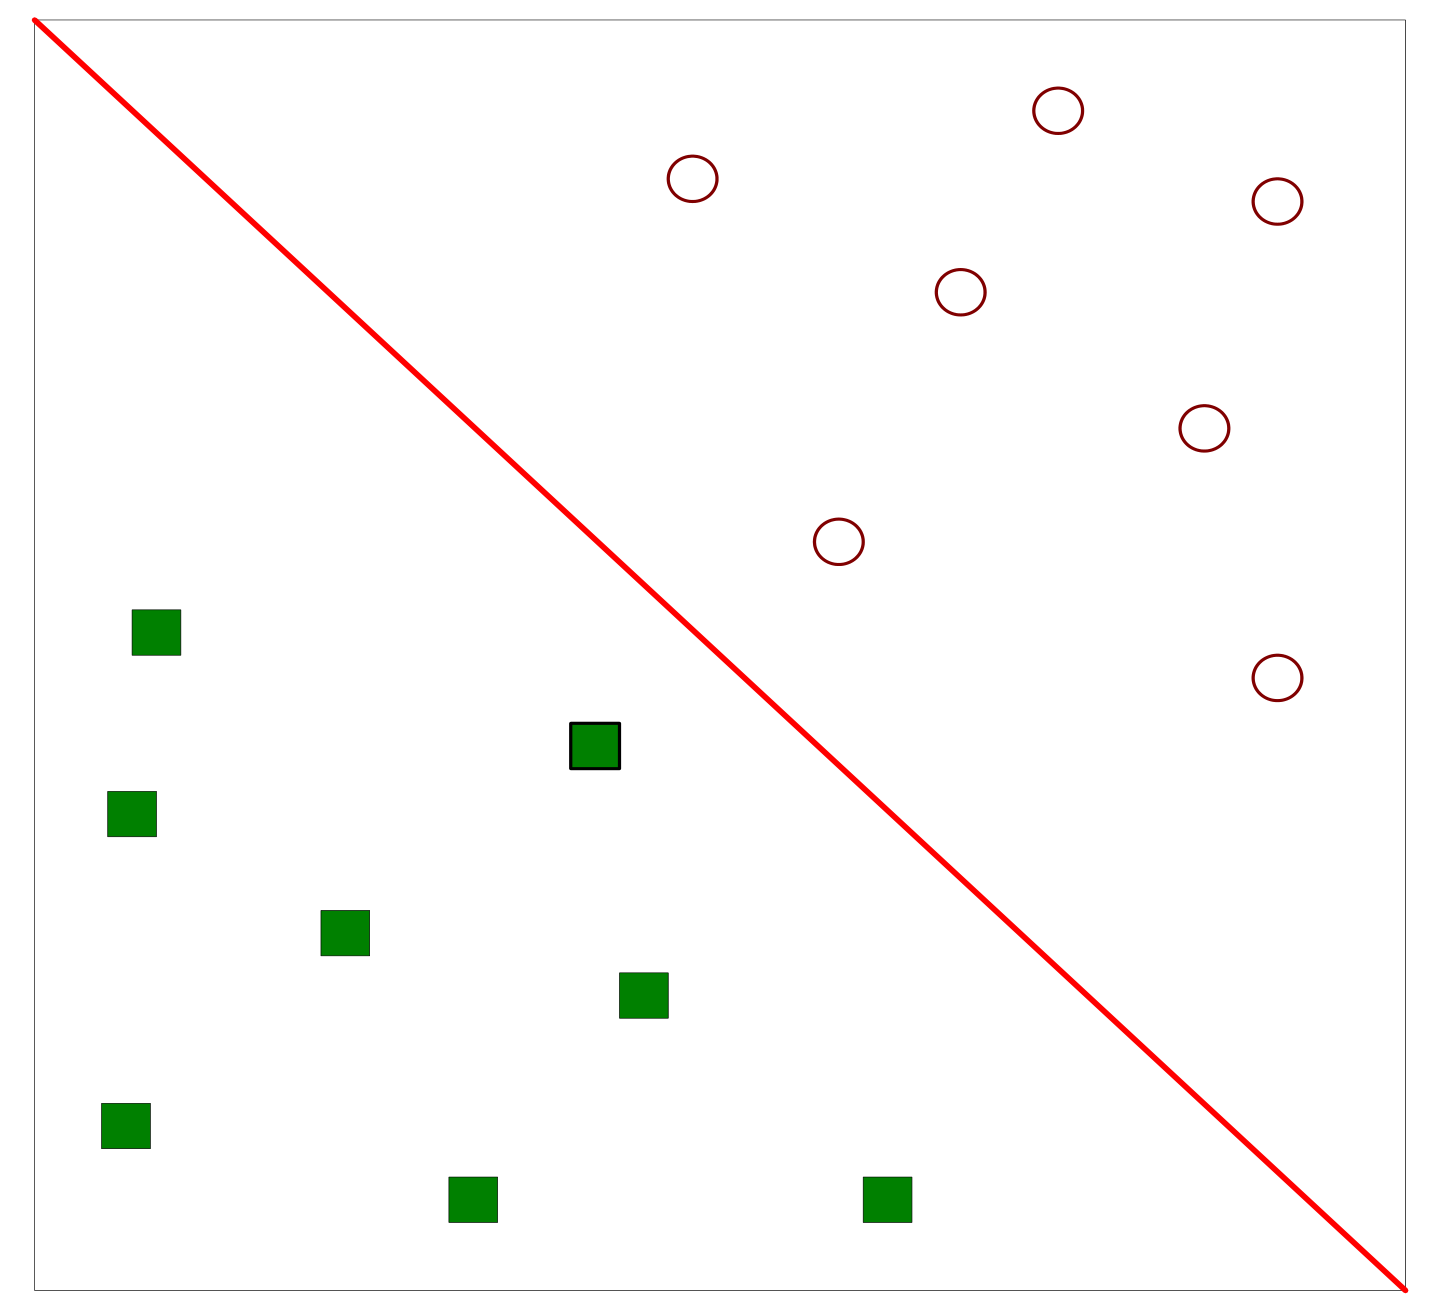
\includegraphics[width=0.55\textwidth,height=5.0cm,keepaspectratio]{images/slide22_svm_linear.png}
  \end{center}
\end{frame}

% Slide 23: Which Hyperplane is better?
\begin{frame}{کدام ابرصفحه برتر است؟}{\lr{Which Hyperplane is better?}}
  \begin{itemize}
    \item کدام ابرصفحه بهتر است؟ $B_1$ یا $B_2$؟ مفهوم «بهتر» چگونه تعریف می‌شود؟
  \end{itemize}
  \vspace{0.1cm}
  \begin{center}
    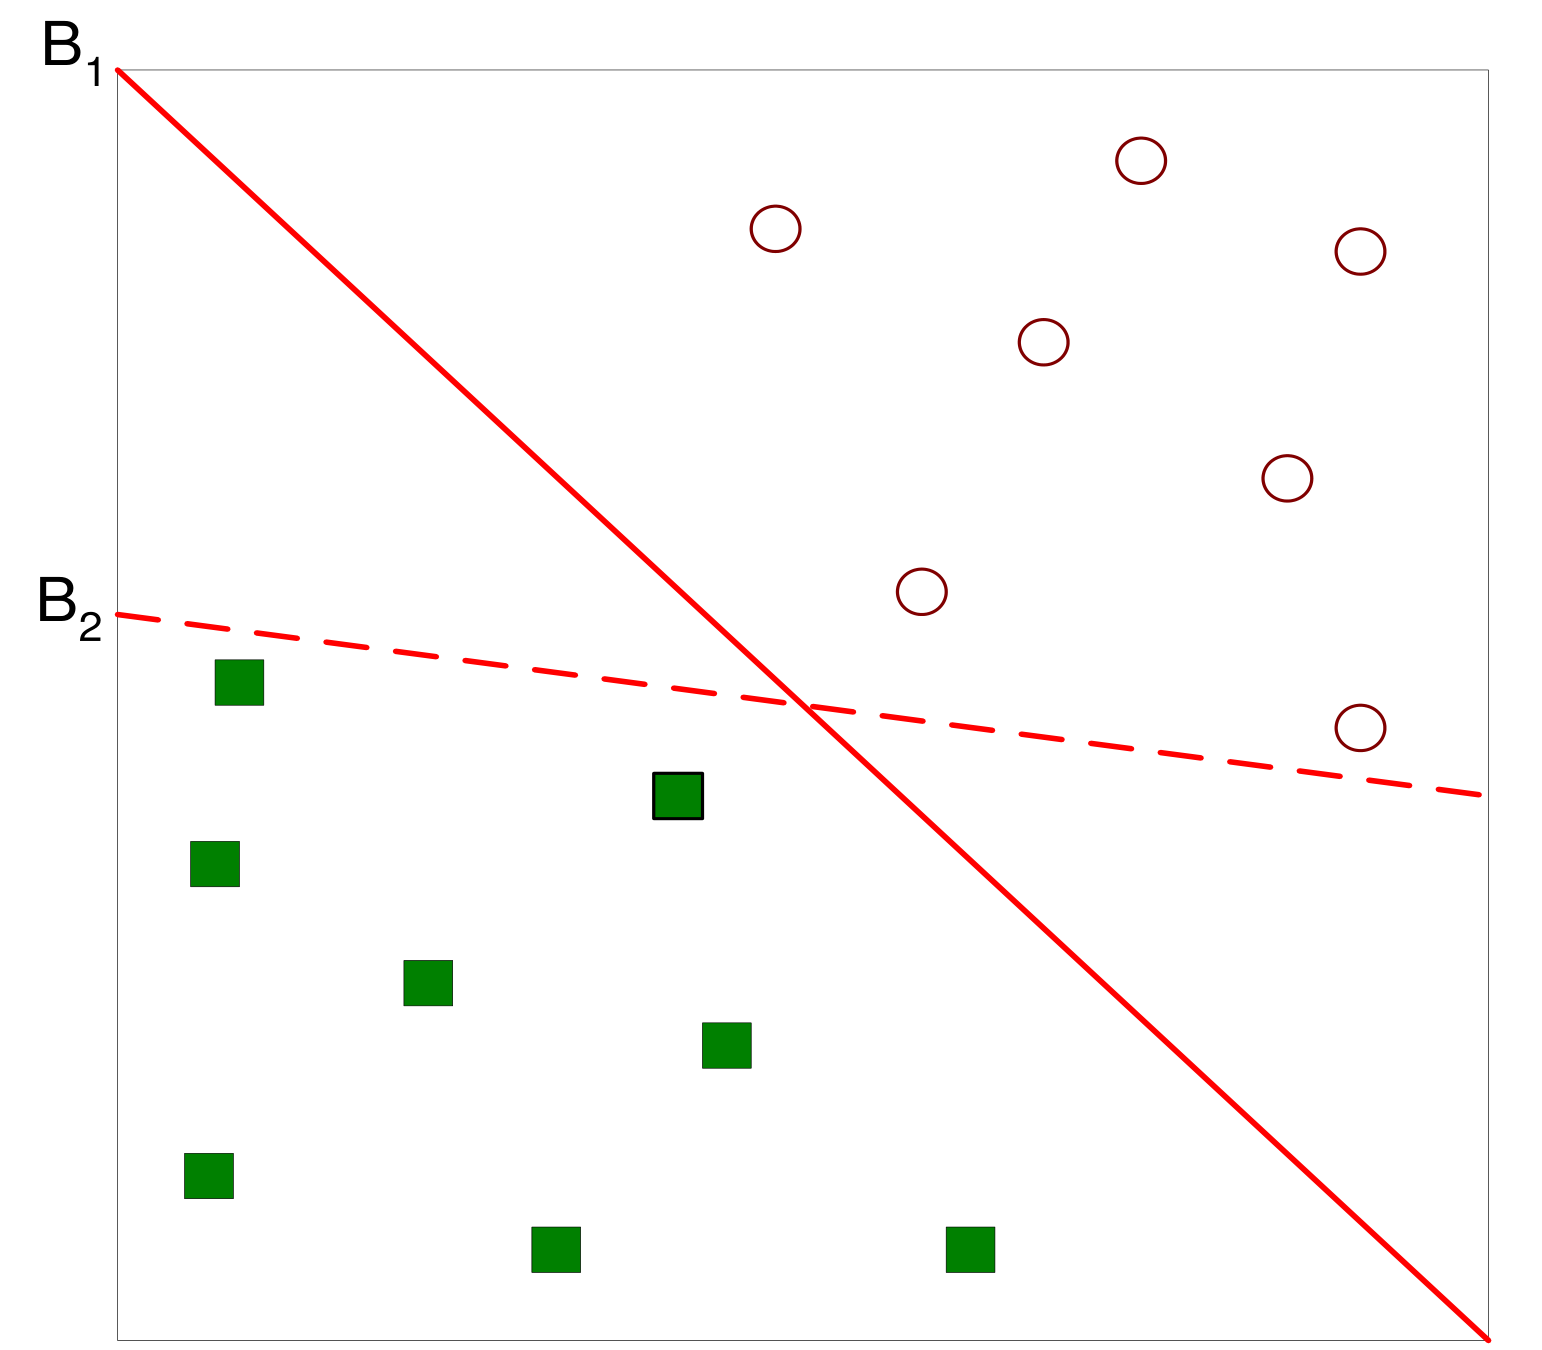
\includegraphics[width=0.55\textwidth,height=5.0cm,keepaspectratio]{images/slide23_svm_b1_b2.png}
  \end{center}
\end{frame}

% Slide 24: Maximal Margin Hyperplane
\begin{frame}{کدام ابرصفحه برتر است؟}{بیشینه‌سازی حاشیه (\lr{Maximal Margin})}
  \begin{itemize}
    \item ابرصفحه‌ای را بیابید که \textbf{حاشیه (\lr{Margin})} تا نزدیک‌ترین نقاط را بیشینه کند تا از بیش‌برازش جلوگیری شود $\implies$ ابرصفحه $B_1$ از $B_2$ برتر است.
  \end{itemize}
  \vspace{0.05cm}
  \begin{center}
    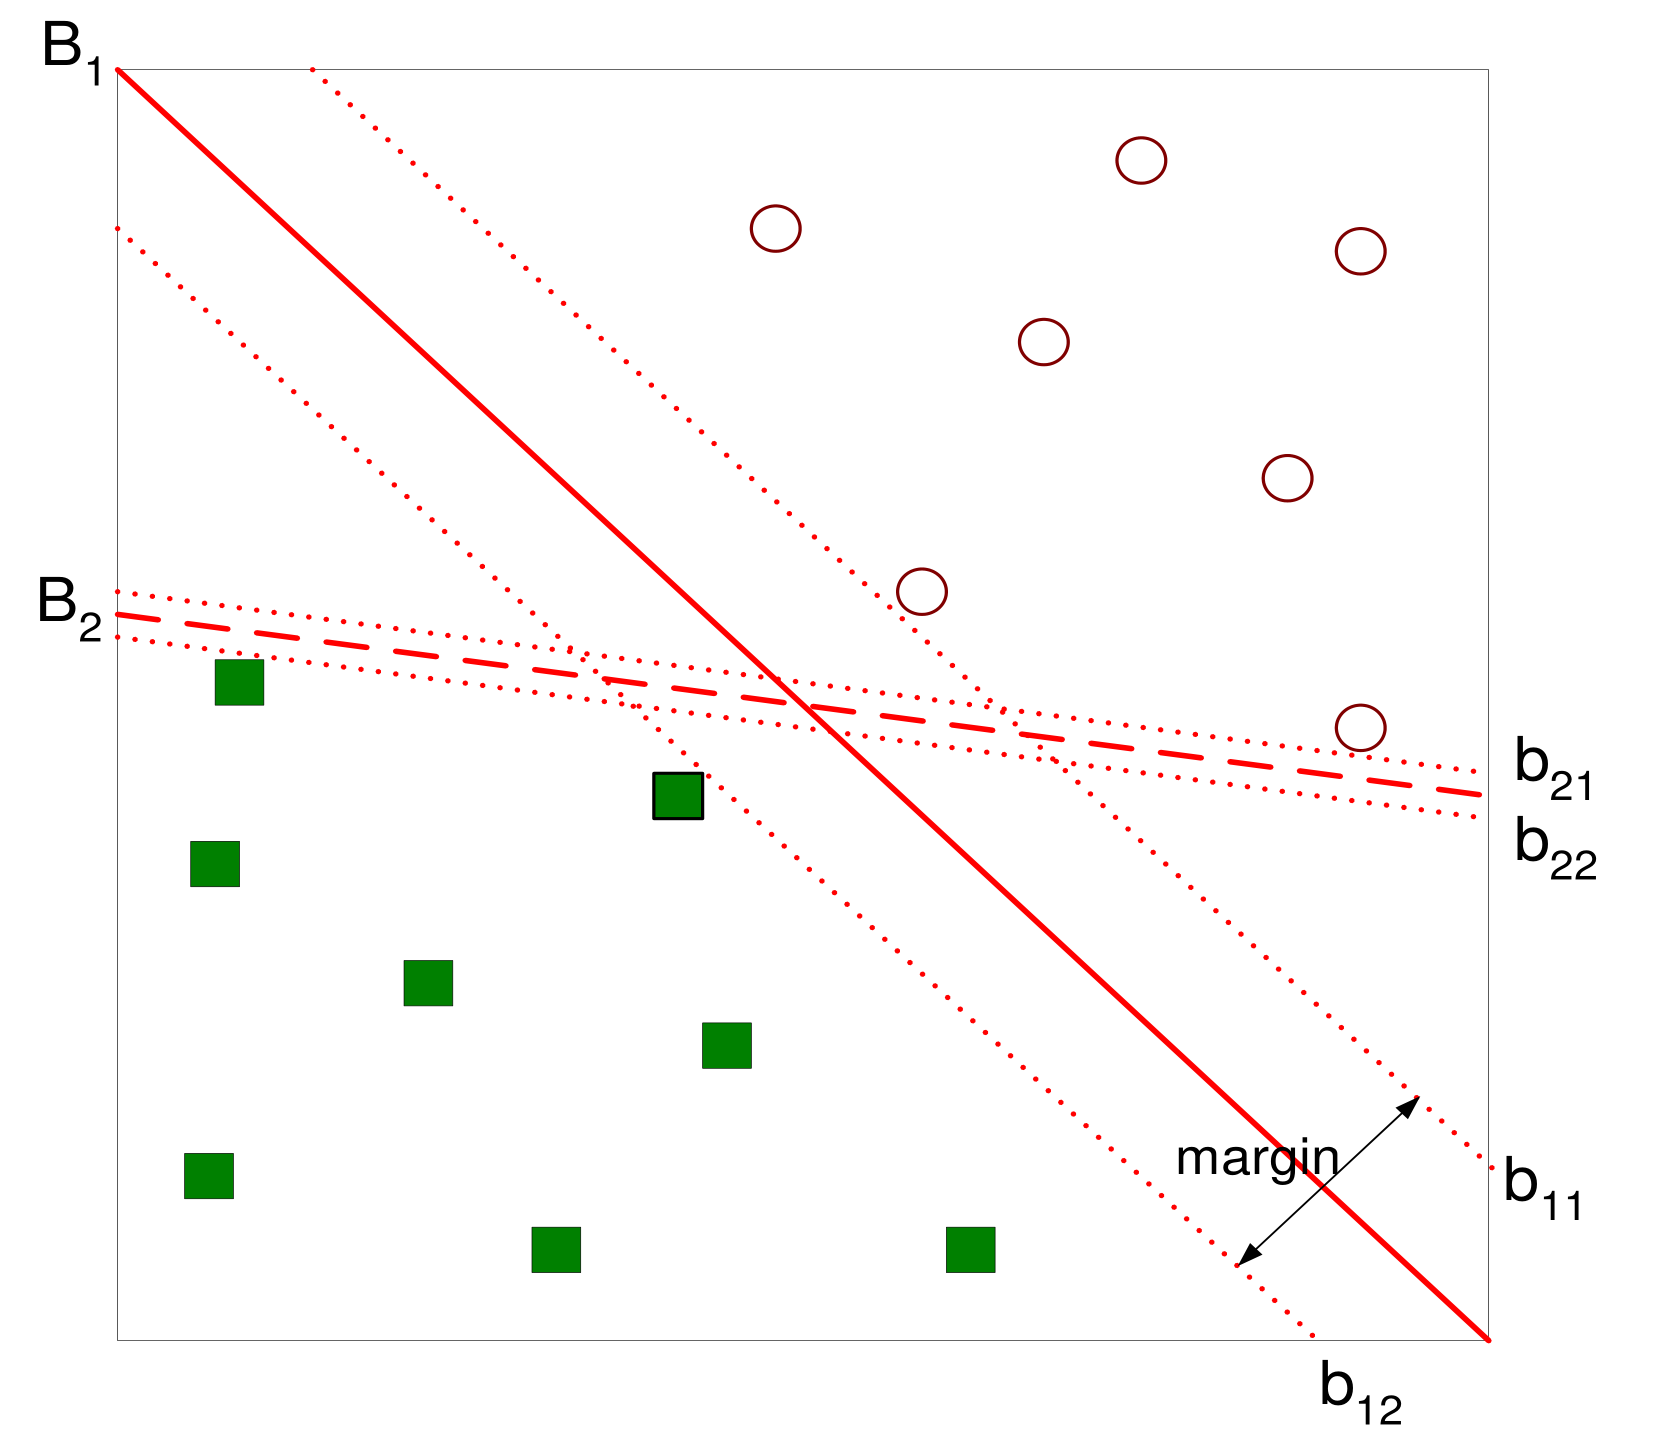
\includegraphics[width=0.55\textwidth,height=5.0cm,keepaspectratio]{images/slide24_svm_margin.png}
  \end{center}
\end{frame}

% Slide 25: Support Vectors
\begin{frame}{کدام ابرصفحه برتر است؟}{نقش بردارهای پشتیبان (\lr{Support Vectors})}
  \begin{itemize}
    \item \textbf{بردارهای پشتیبان} (\lr{Support Vectors}): نزدیک‌ترین نقاط آموزشی به ابرصفحه تصمیم هستند که موقعیت و جهت مرز تصمیم را به طور کامل تعیین می‌کنند.
  \end{itemize}
  \vspace{0.05cm}
  \begin{center}
    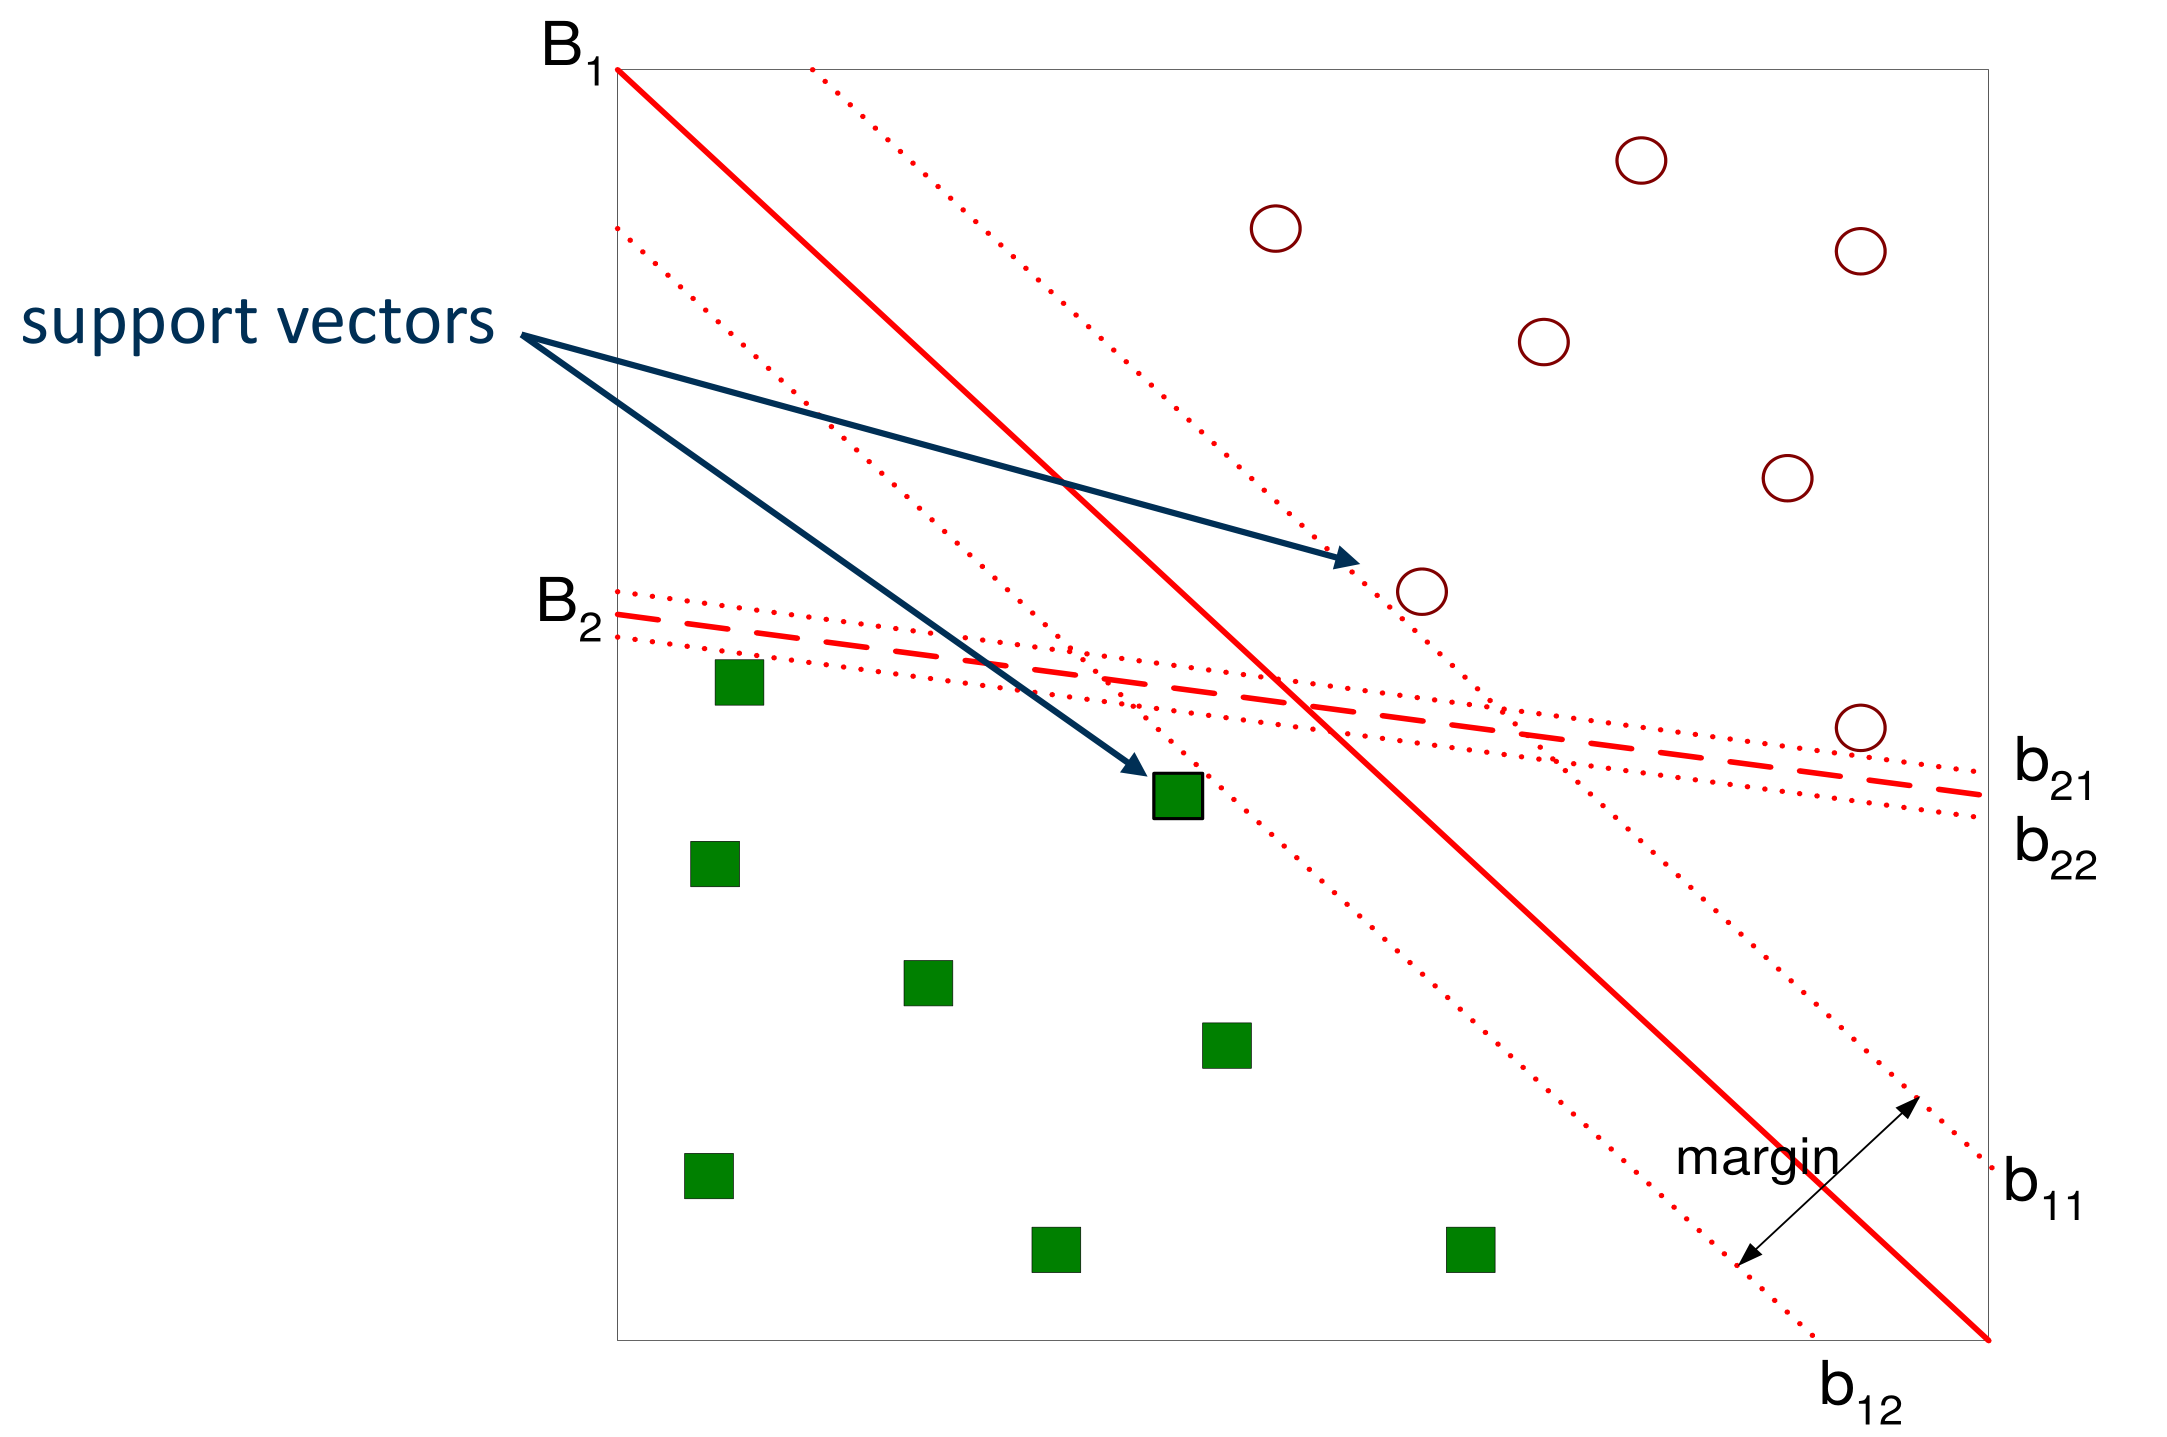
\includegraphics[width=0.62\textwidth,height=5.0cm,keepaspectratio]{images/slide25_svm_support_vectors.png}
  \end{center}
\end{frame}

% Slide 26: Soft Margin & Slack Variables
\begin{frame}{داده‌های تفکیک‌ناپذیر خطی}{متغیرهای کمکی (\lr{Slack Variables}) و حاشیه نرم}
  \begin{itemize}
    \setlength{\itemsep}{6pt}
    \item در صورت هم‌پوشانی داده‌ها یا وجود نویز، تفکیک خطی محض ممکن نیست.
    \item \textbf{راه‌حل:} معرفی \textbf{متغیرهای کمکی ($\xi_i$)} در رابطه بهینه‌سازی که برای هر نمونه ناقض مرز جریمه تعیین می‌کند.
  \end{itemize}
  \vspace{0.05cm}
  \begin{center}
    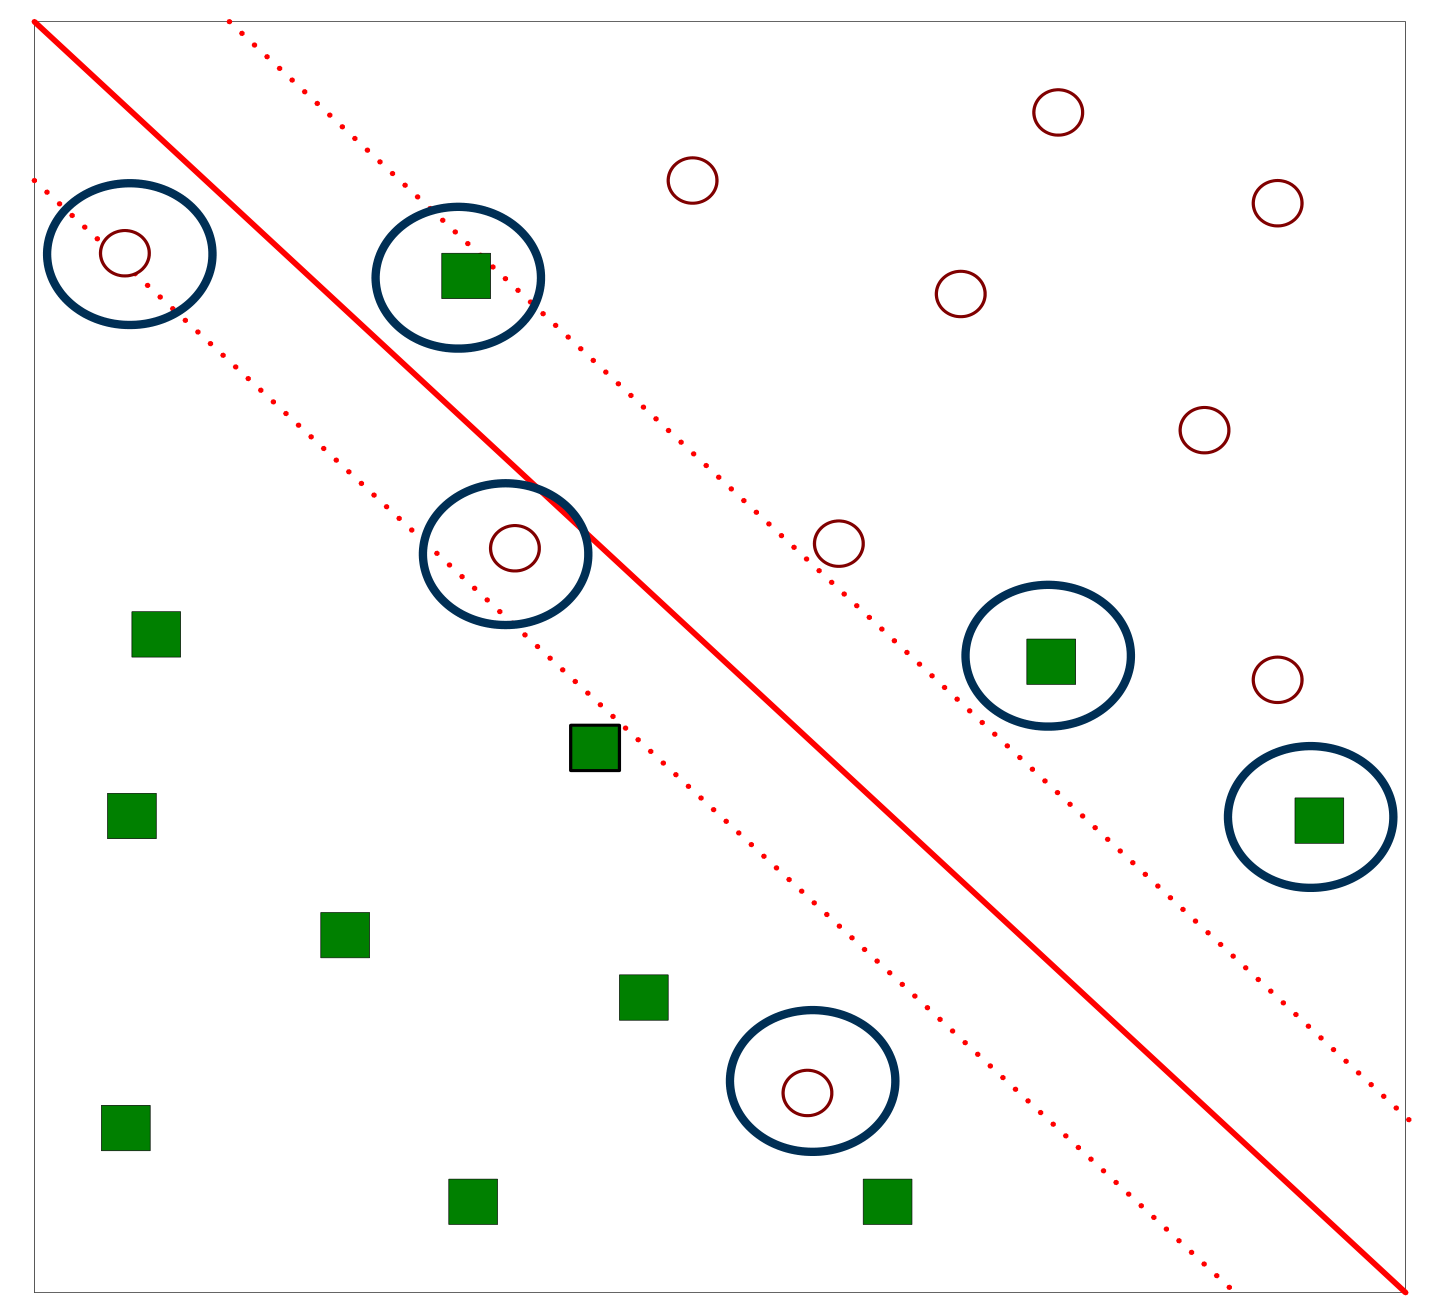
\includegraphics[width=0.55\textwidth,height=4.8cm,keepaspectratio]{images/slide26_svm_slack.png}
  \end{center}
\end{frame}

% Slide 27: Nonlinear SVM - Intro
\begin{frame}{ماشین‌های بردار پشتیبان غیرخطی}{چالش مرزهای غیرخطی}
  \begin{itemize}
    \item چه رخ می‌دهد اگر مرز تصمیم در فضای ویژگی‌ها ذاتاً غیرخطی باشد؟
  \end{itemize}
  \vspace{0.15cm}
  \begin{center}
    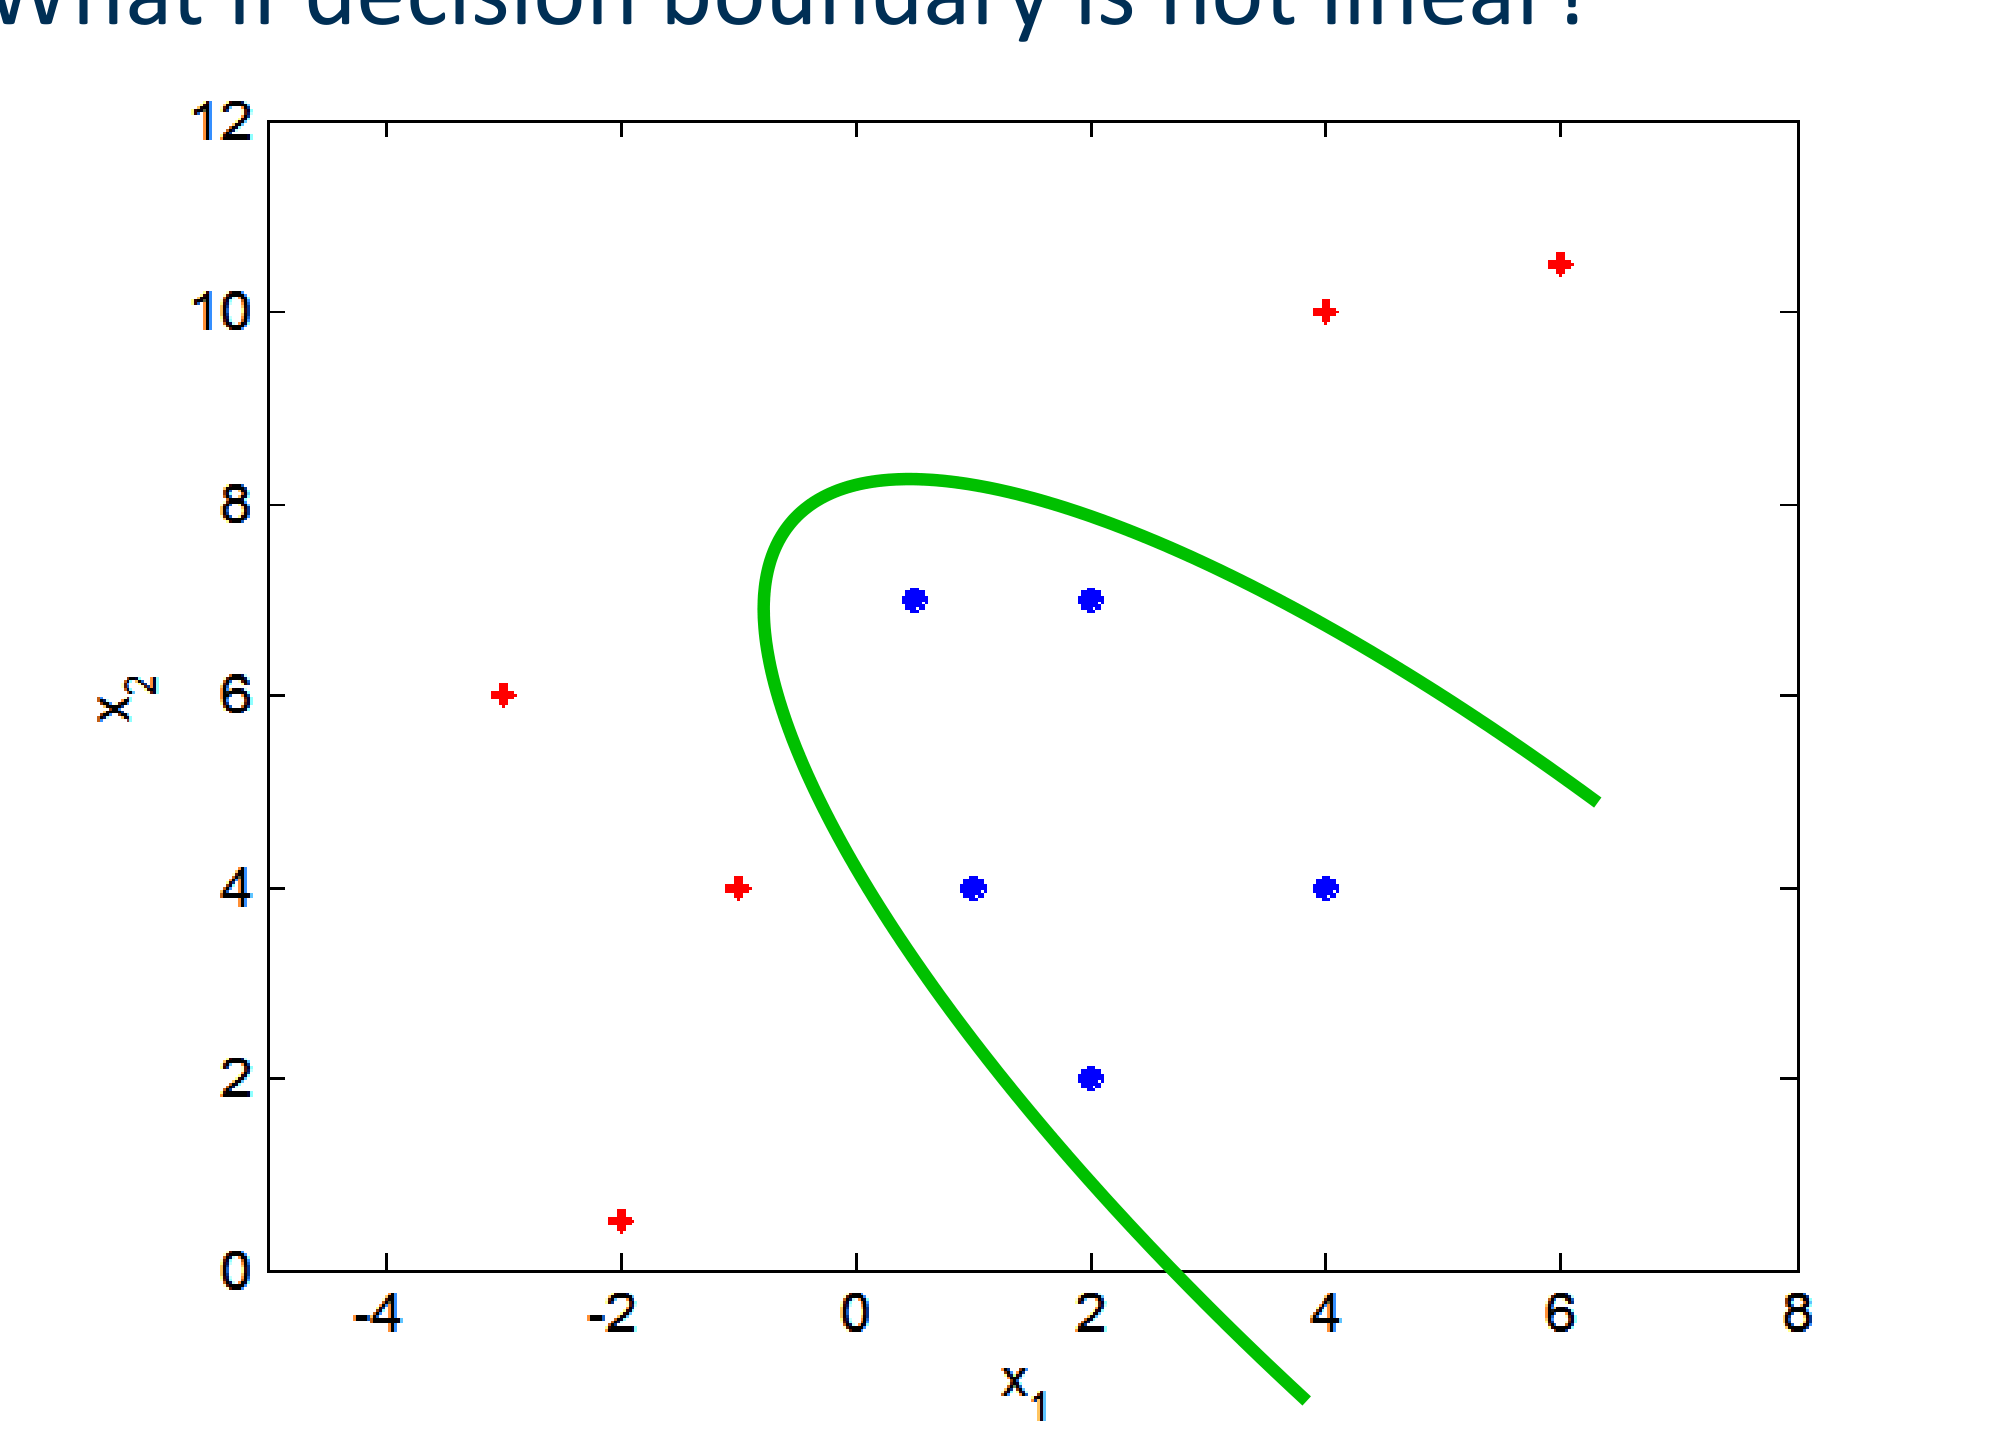
\includegraphics[width=0.75\textwidth,height=4.8cm,keepaspectratio]{images/slide27_nonlinear_svm_circle.png}
  \end{center}
\end{frame}

% Slide 28: Transformation to Higher Dimensional Space
\begin{frame}{نگاشت به فضای با ابعاد بالاتر}{\lr{Feature Space Transformation}}
  \begin{itemize}
    \item نگاشت داده‌های غیرقابل تفکیک خطی در فضای اولیه به یک فضای ابعاد بالاتر با تابع $\Phi(x)$ که در آن داده‌ها به صورت خطی جداپذیر می‌گردند.
  \end{itemize}
  \vspace{0.15cm}
  \begin{center}
    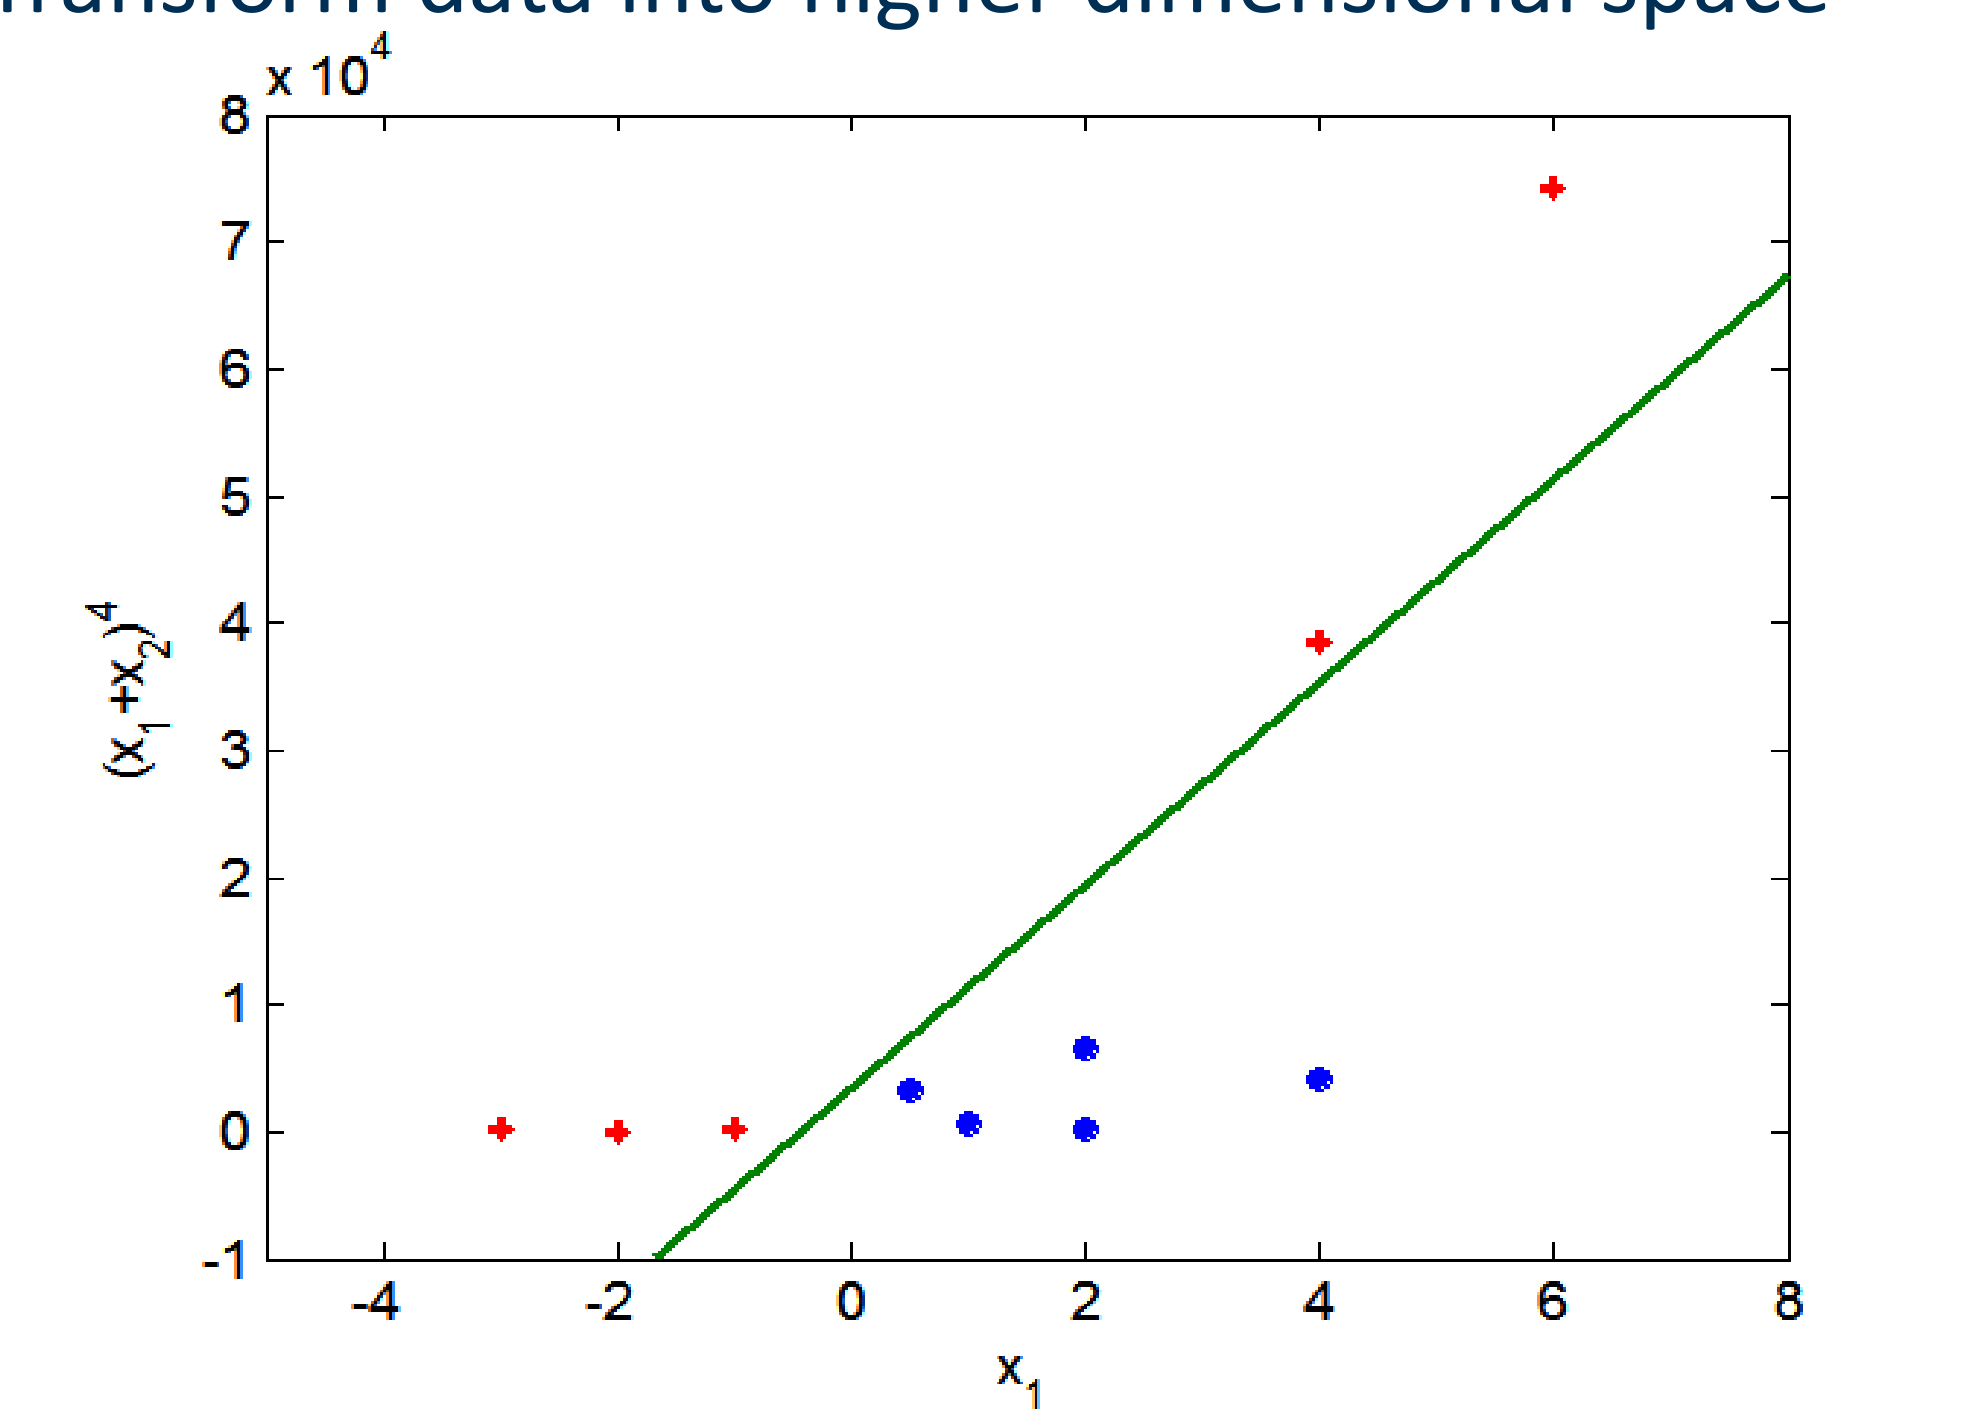
\includegraphics[width=0.75\textwidth,height=4.8cm,keepaspectratio]{images/slide28_nonlinear_mapping.png}
  \end{center}
\end{frame}

% Slide 29: Kernel Trick & Python Implementation
\begin{frame}{ترفند کرنل و پیاده‌سازی پایتون}{\lr{The Kernel Trick \& Scikit-learn}}
  \begin{itemize}
    \setlength{\itemsep}{5pt}
    \item نگاشت صریح به فضای ابعاد بالا از نظر محاسباتی بسیار سنگین است.
    \item \textbf{ترفند کرنل} (\lr{Kernel Trick}): محاسبات ضرب داخلی مستقیماً در همان فضای ابعاد پایین با تابع کرنل انجام می‌شود ($K(x, z) = \langle\Phi(x), \Phi(z)\rangle$).
    \begin{itemize}
      \item انواع توابع کرنل رایج: چندجمله‌ای (\lr{Polynomial})، پایه شعاعی گاوسی (\lr{RBF}).
    \end{itemize}
    \item \textbf{پیاده‌سازی در پایتون} (\lr{scikit-learn}):
  \end{itemize}
  \vspace{0.15cm}
  \begin{latin}
    \begin{minipage}{0.96\textwidth}
      \fcolorbox{codeborder}{codebg}{%
        \begin{minipage}{0.97\textwidth}
          \ttfamily\small
          \textcolor{mannheimteal}{\# Import Support Vector Classifier}\\
          \textbf{from} sklearn.svm \textbf{import} SVC\\[4pt]
          \textcolor{mannheimteal}{\# Train SVM classifier with RBF kernel and penalty C=1.0}\\
          estimator = SVC(C=1.0, kernel=\textcolor{teal}{'rbf'})\\[2pt]
          estimator.fit(scaled\_training\_data, training\_labels)
        \end{minipage}%
      }
    \end{minipage}
  \end{latin}
\end{frame}

% Slide 30: Tuning of SVM
\begin{frame}{تنظیم سیستماتیک فراپارامترهای الگوریتم \lr{SVM}}{\lr{Systematic SVM Parameter Tuning}}
  \begin{itemize}
    \setlength{\itemsep}{5pt}
    \item به جای آزمون تصادفی چند کرنل و پارامتر، هسو و همکاران روشی سیستماتیک پیشنهاد می‌دهند:
    \begin{enumerate}
      \setlength{\itemsep}{3pt}
      \item \textbf{مقیاس‌بندی خطی} تمام ویژگی‌ها در بازه $[-1, +1]$ یا $[0, 1]$.
      \item استفاده از \textbf{کرنل پایه شعاعی} (\lr{RBF Kernel}).
      \item \textbf{اعتبارسنجی متقاطع} برای یافتن بهترین مقادیر $C$ و $\gamma$ در دنباله‌های با رشد نمایی:
      \[
        C \in \{2^{-5}, 2^{-3}, \dots, 2^{15}\}, \quad \gamma \in \{2^{-15}, 2^{-13}, \dots, 2^3\}
      \]
      \item آموزش مدل نهایی روی کل داده‌های آموزش با بهترین مقادیر $C$ و $\gamma$.
      \item \textbf{ارزیابی نهایی} روی مجموعه آزمون (\lr{Test}).
    \end{enumerate}
  \end{itemize}
  \vfill
  {\fontsize{7}{8.5}\selectfont\color{subgray}
    \lr{Chih-Wei Hsu, Chih-Chung Chang, and Chih-Jen Lin: A Practical Guide to Support Vector Classification}
  }
\end{frame}
